
% Programming/Coding Assignment
% LaTeX Template
%
% This template has been downloaded from:
% http://www.latextemplates.com
%
% Original author:
% Ted Pavlic (http://www.tedpavlic.com)
%
% Note:
% The \lipsum[#] commands throughout this template generate dummy text
% to fill the template out. These commands should all be removed when 
% writing assignment content.
%
% This template uses a Perl script as an example snippet of code, most other
% languages are also usable. Configure them in the "CODE INCLUSION 
% CONFIGURATION" section.
%
%%%%%%%%%%%%%%%%%%%%%%%%%%%%%%%%%%%%%%%%%

%----------------------------------------------------------------------------------------
%   PACKAGES AND OTHER DOCUMENT CONFIGURATIONS
%----------------------------------------------------------------------------------------

\documentclass{article}

\usepackage{fancyhdr} % Required for custom headers
\usepackage{lastpage} % Required to determine the last page for the footer
\usepackage{extramarks} % Required for headers and footers
\usepackage[usenames,dvipsnames]{color} % Required for custom colors
\usepackage{graphicx} % Required to insert images
\usepackage{listings} % Required for insertion of code
\usepackage{courier} % Required for the courier font
\usepackage{lipsum} % Used for inserting dummy 'Lorem ipsum' text into the template
\usepackage{multicol}
\usepackage{fullpage,amsthm,amsfonts,amssymb,epsfig,amsmath}

% Margins
\topmargin=-0.45in
\evensidemargin=0in
\oddsidemargin=0in
\textwidth=6.5in
\textheight=9.0in
\headsep=0.25in

\linespread{1.1} % Line spacing

% Set up the header and footer
\pagestyle{fancy}
\lhead{\hmwkAuthorName} % Top left header
\chead{\hmwkClass\ (\hmwkClassInstructor\ \hmwkClassTime): \hmwkTitle} % Top center head
\rhead{\firstxmark} % Top right header
\lfoot{\lastxmark} % Bottom left footer
\cfoot{} % Bottom center footer
\rfoot{Page\ \thepage\ of\ \protect\pageref{LastPage}} % Bottom right footer
\renewcommand\headrulewidth{0.4pt} % Size of the header rule
\renewcommand\footrulewidth{0.4pt} % Size of the footer rule
\newcommand{\tab}{\hspace*{3em}}

\setlength\parindent{0pt} % Removes all indentation from paragraphs

%----------------------------------------------------------------------------------------
%   CODE INCLUSION CONFIGURATION
%----------------------------------------------------------------------------------------

\definecolor{MyDarkGreen}{rgb}{0.0,0.4,0.0} % This is the color used for comments
\lstloadlanguages{Perl} % Load Perl syntax for listings, for a list of other languages supported see: ftp://ftp.tex.ac.uk/tex-archive/macros/latex/contrib/listings/listings.pdf
\lstset{language=Perl, % Use Perl in this example
        frame=single, % Single frame around code
        basicstyle=\small\ttfamily, % Use small true type font
        keywordstyle=[1]\color{Blue}\bf, % Perl functions bold and blue
        keywordstyle=[2]\color{Purple}, % Perl function arguments purple
        keywordstyle=[3]\color{Blue}\underbar, % Custom functions underlined and blue
        identifierstyle=, % Nothing special about identifiers                                         
        commentstyle=\usefont{T1}{pcr}{m}{sl}\color{MyDarkGreen}\small, % Comments small dark green courier font
        stringstyle=\color{Purple}, % Strings are purple
        showstringspaces=false, % Don't put marks in string spaces
        tabsize=5, % 5 spaces per tab
        %
        % Put standard Perl functions not included in the default language here
        morekeywords={rand},
        %
        % Put Perl function parameters here
        morekeywords=[2]{on, off, interp},
        %
        % Put user defined functions here
        morekeywords=[3]{test},
        %
        morecomment=[l][\color{Blue}]{...}, % Line continuation (...) like blue comment
        numbers=left, % Line numbers on left
        firstnumber=1, % Line numbers start with line 1
        numberstyle=\tiny\color{Blue}, % Line numbers are blue and small
        stepnumber=5 % Line numbers go in steps of 5
}

% Creates a new command to include a perl script, the first parameter is the filename of the script (without .pl), the second parameter is the caption
\newcommand{\perlscript}[2]{
\begin{itemize}
\item[]\lstinputlisting[caption=#2,label=#1]{#1.pl}
\end{itemize}
}

%----------------------------------------------------------------------------------------
%   DOCUMENT STRUCTURE COMMANDS
%   Skip this unless you know what you're doing
%----------------------------------------------------------------------------------------

% Header and footer for when a page split occurs within a problem environment
\newcommand{\enterProblemHeader}[1]{
\nobreak\extramarks{#1}{#1 continued on next page\ldots}\nobreak
\nobreak\extramarks{#1 (continued)}{#1 continued on next page\ldots}\nobreak
}

% Header and footer for when a page split occurs between problem environments
\newcommand{\exitProblemHeader}[1]{
\nobreak\extramarks{#1 (continued)}{#1 continued on next page\ldots}\nobreak
\nobreak\extramarks{#1}{}\nobreak
}

\setcounter{secnumdepth}{0} % Removes default section numbers
\newcounter{homeworkProblemCounter} % Creates a counter to keep track of the number of problems

\newcommand{\homeworkProblemName}{}
\newenvironment{homeworkProblem}[1][Problem \arabic{homeworkProblemCounter}]{ % Makes a new environment called homeworkProblem which takes 1 argument (custom name) but the default is "Problem #"
\stepcounter{homeworkProblemCounter} % Increase counter for number of problems
\renewcommand{\homeworkProblemName}{#1} % Assign \homeworkProblemName the name of the problem
\section{\homeworkProblemName} % Make a section in the document with the custom problem count
\enterProblemHeader{\homeworkProblemName} % Header and footer within the environment
}{
\exitProblemHeader{\homeworkProblemName} % Header and footer after the environment
}

\newcommand{\problemAnswer}[1]{ % Defines the problem answer command with the content as the only argument
\noindent\framebox[\columnwidth][c]{\begin{minipage}{0.98\columnwidth}#1\end{minipage}} % Makes the box around the problem answer and puts the content inside
}

\newcommand{\homeworkSectionName}{}
\newenvironment{homeworkSection}[1]{ % New environment for sections within homework problems, takes 1 argument - the name of the section
\renewcommand{\homeworkSectionName}{#1} % Assign \homeworkSectionName to the name of the section from the environment argument
\subsection{\homeworkSectionName} % Make a subsection with the custom name of the subsection
\enterProblemHeader{\homeworkProblemName} % Header and footer within the environment
}{
\enterProblemHeader{\homeworkProblemName} % Header and footer after the environment
}

%----------------------------------------------------------------------------------------
%   NAME AND CLASS SECTION
%----------------------------------------------------------------------------------------

\newcommand{\hmwkTitle}{Homework\ \#7} % Assignment title
\newcommand{\hmwkDueDate}{Tuesday,\ May\ 26th,\ 2015} % Due date
\newcommand{\hmwkClass}{CMPS\ 102} % Course/class
\newcommand{\hmwkClassTime}{4:00pm} % Class/lecture time
\newcommand{\hmwkClassInstructor}{Warmuth} % Teacher/lecturer
\newcommand{\hmwkAuthorName}{John Allard \ 1437547
} % Your name


%----------------------------------------------------------------------------------------
%----------------------------------------------------------------------------------------
%   USER SETTINGS
%----------------------------------------------------------------------------------------
%----------------------------------------------------------------------------------------
\usepackage{mathtools}
\DeclarePairedDelimiter\ceil{\lceil}{\rceil}
\DeclarePairedDelimiter\floor{\lfloor}{\rfloor}



%----------------------------------------------------------------------------------------
%   TITLE PAGE
%----------------------------------------------------------------------------------------

\title{
\vspace{2in}
\textmd{\textbf{\hmwkClass:\ \hmwkTitle}}\\
\normalsize\vspace{0.1in}\small{Due\ on\ \hmwkDueDate}\\
\vspace{0.1in}\large{\textit{}}
\vspace{3in}
}

\author{\textbf{\hmwkAuthorName}}
\date{} % Insert date here if you want it to appear below your name

%----------------------------------------------------------------------------------------

\begin{document}

\maketitle

%----------------------------------------------------------------------------------------
%   TABLE OF CONTENTS
%----------------------------------------------------------------------------------------

%\setcounter{tocdepth}{1} % Uncomment this line if you don't want subsections listed in the ToC

% \tableofcontents
\newpage





%----------------------------------------------------------------------------------------
%   PROBLEM 1
%----------------------------------------------------------------------------------------

% To have just one problem per page, simply put a \clearpage after each problem

\begin{homeworkProblem}
1) Consider the longest common subsequence problem between two strings $x_1,...,x_n$ and $y_1,...,y_m$. Define a graph over the nxm grid (plus possibly some vertices around the edges) s.t. the longest common subsequence corresponds to the longest path in this graph.
- Clearly describe the condition for the presence of an edge between two vertices on the grid. \\
- How should the edges be labeled? \\
- How do you find the longest path? \\
- Is this algorithm more efficient than the dynamic programming algorithm? \\

\textbf{Answer : }
We will solve this problem using a directed graph over $m \times n$ vertices that are labeled according to their coordinates $(p,q)$ : $0 \leq p \leq m$ and $0 \leq q \leq n$. Edges are generated as follows :
if letters $p$ and $q$ are the same, draw an edge from $V(p, q)$ to $V(p+1, q+1)$, aka a diagonal. If the letters are different, draw two edges from $V(p, q)$, one to $V(p+1, q)$ and the other to $V(p, q+1)$, aka down and right. The import part is this : edges that go diagonal are given a weight of 1, and edges that go right or down get a weight of 0. The longest path now doens't depend on the number of edges directly, but rather how many diagonal edges are along a path, since they contribute all of the weight.  \\

\begin{multicols}{2}
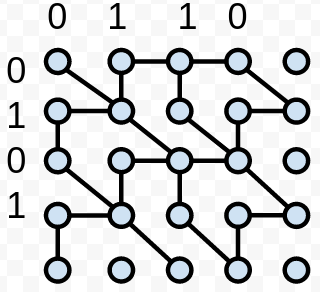
\includegraphics[scale=0.7]{p1_graph.png} \\
Graph of \texttt{0101} and \texttt{0110}.
\columnbreak \\
Because all edges travel in either the positive x, positive y, or positive x and y directions, we know that this graph is acyclic. Because this graph is directed and acyclic, we can use a realtively fast algorithm (compared to the NP-hard algorithm for the longest-path on a general-graph case) to find the longest path. The algorithm contains two parts, making the graph and retreiving the longest path. To find the longest path, we have to find a topological sort of the graph. \\
This can be done with a modifed version of DFS that pushes vertices onto a stack, at the very end that stack will contain the topological sort of G. Once we have this sort, we can find the longest path using a simple algorithm. \\ 
\end{multicols}

Start by walking over all $m \times n$ vertices in the graph and generating edges. Each vertex can have at most two edges eminated from it, so each of the $m \times n$ operation are constant. Thus constructing the graph is $O(mn)$. Once the graph is constructed, DFS is run on it which runs in time $O(|V+E|)$, since $E \leq 2*|V|$, DFS runs in time $O(|V|) = O(mn)$. DFS gives us our topoligical sort, which leads to the last portion of our algorithm, retreiving the longest path. \\
The algorithm in short walks along the topolical sort from the source vertex (which would be $V(0, 0)$ for the shortest-common-subsequence problem), and updates its neighbors where-ever it can by adding its own weight-sum to the weight of the incident edges and setting the neighbors weight-sum to this value. 
\end{homeworkProblem}






%----------------------------------------------------------------------------------------
%   PROBLEM 2
%----------------------------------------------------------------------------------------

\begin{homeworkProblem}
 Suppose we are given three strings of characters $X = x_1 x_2 ... x_m$, $Y = y_1 y_2 ... y_n$, and $Z = z_1 z_2 ... z_m+n$. $Z$ is said to be a "shuffle" of $X$ and $Y$ if $Z$ can be formed by interspersing the characters from $X $and $Y$ in a way that maintains to left-to-right ordering of the characters from each string. For example the, cchocohilaptes is a shuffle of chocolate and chips,  but chocochilatspe is not. Devise a dynamic programming algorithm that takes as input $X$,$Y$,$Z$,$m$, and $n$, and determines whether or not $Z$ is a shuffle of $X$ and $Y$. Analyze the worst-case running time and space requirements of your algorithm.  \\

Hint: The values in your table should be Boolean, not numeric.

\textbf{Answer : } \\
The algorithm to solve this problem will depend on 2 variables, the indices of the characters in $X$ and $Y$. We can calculate the index of the character we're comparing for the current iteration in $Z$ by adding the indices of the current characters we're looking at it and $X$ and $Y$ and subtracting one. \\ 
The subproblems are as follows : If the current problem is on the strings $X[1:i]$, $Y[1:j]$, $Z[1:k] k = i+j-1$, the subproblems consist of seeing if the strings $Z[1:k-1], X[1:i-1], Y[1:j]$ or $Z[1:k-1], X[1:i], Y[1:j-1]$ are shuffles of one another. Given the answer to these subproblems, we can find the solution to the current-length strings by seeing if the character $Z_k$ can be made by taking either $X_i$ or $Y_j$ and combining it with the answers to the 2 subproblems. This will be made specific below. \\
The table in this case is boolean (as was suggested in the hint), with dimensions $m \times n$ The bool in table entry $(i,j)$ represents if the either of the characters $X_i$ or $Y_j$ can be used to make the character $Z_k : k = i+j-1$. The arrows for this table either go right or left, depending on which string has the character that matches the character in $Z$. If $Z_k$ is matches by a character on the $x$ axis, we travel left, if it is matches by a character on the $y$ axis we go up, and if they both match we can go either way. \\

The formal recurrance relation is as follows : Given strings $X$ of length $m$, $Y$ of length $n$, and $Z$ of length $n+m$, $S(p, q) : (m,n) \geq (p,q) \geq (0,0) $ takes the indices of two characters in $X$ and $Y$ and returns a boolean value. $S$ is defined as :
$$ S(p, q) = [(Z_k === X_p \text{ AND } S(p-1, q)) \text{ OR } (Z_k == Y_q \text{ AND } S(p, q-1)) ] $$

We also have the base cases that if $p$ or $q$ becomes $0$, we simply check other non-zero index. If they're both zero we return true. \\

This says that at index $k = p+q$, we either match the character $X_p$ and recurse on $Z$ with one less character, $X$ with one less character, and $Y$ as it is, or we do the same except with $Y$. 

The algorithm doesn't actually need to build the algoritmh
% To build the table with the algorithm, we work our way up from entry $(1,1)$. If we match a character on the horizontal axis, we travel right, if we match a character on the vertical axis, we travel down. We continue until we evaluate thee entry $(m,n)$, because this is the case where we are looking at the last letter in $Z$ which is at index $k= m+n$.

\begin{lstlisting}
# X, Y, Z = strings of len (m, n, m+n-1)
# @args - p, q are the X, Y indices we are currently querying.
checkShuffle(M, X, Y, Z) :
  p = 1
  q = 1
  # note the short-circuit AND evalutation to avoid indexing out of X or Y
  while (p+q) < (m+n) :
    k = p+q-1
    if p <= m AND Z[k] == X[p] :
      p = p+1
    else if q <= n AND Z[k] == Y[q] :
      q = q+1
    else :
      return false

  return true
\end{lstlisting}

The running time for this algorithm is linear in $m$ and $n$, which means it is linear in the size of $Z$. If this was the strictly harder version of this problem where a matching character in $Z$ and count for both a match in $X$ and $Y$ is a strictly harder problem and wouldn't be able to be solved so easily. Notice the algorithm doesn't even need to fill in the table, it can find a path through it without needing to fill in the entire thing. This is because once it finds the character $X_p$ cannot match at position $Z_k$, it knows that no character $X_{p+n} : n > 0$ can be placed in the spot either without violating the ordering of $X$. The algorithm runs a single for-loop from iteration number 1 to iteration $k$, increasing by one each time. If it runs into a wall it returns false right away.

\end{homeworkProblem}



\newpage

%----------------------------------------------------------------------------------------
%   PROBLEM 3
%----------------------------------------------------------------------------------------
\begin{homeworkProblem}

\vspace{2mm}

Suppose that you are given an n x n checkerboard and a
checker. You must move the checker from the bottom edge of
the board to the top edge of the board according to the
following rule. At each step you may move the checker to one
of three squares:

\begin{enumerate} 
  \item the square immediately above,
  \item the square that is one up and one to the left (but only if the checker is not already in the leftmost column).
  \item the square that is one up and one to the right (but only if the checker is not already the rightmost column).
\end{enumerate}

Each time you move form square x to square y, you receivep(x,y) dollars. Your are given p(x,y) for all pairs (x,y) for which a move from x to y is legal. Do not assume that p(x,y) is positive. \\
Give an algorithm that figures out the set of moves that will move the checker from somewhere along the bottom edge to somewhere along the top edge while gathering as many dollars as possible. Your algorithm is free to pick any square along the bottom edge as a starting point and any square along the top edge as a destination in order to maximize the number of dollars gathering along the way. What is the running time of your algorithm?


\end{homeworkProblem}


\newpage


%----------------------------------------------------------------------------------------
%   PROBLEM 4
%----------------------------------------------------------------------------------------
\begin{homeworkProblem}

Extra Credit:
Viterbi algorithm.We can use dynamic programming on a directed graph $G=(V,E)$for speech recognition. Each edge $(u,v)$ in $E$ is labeledwith a sound $s(u,v)$ from a finite set $S$ of sounds. Thelabeled graph is a formal model of a person speaking arestricted language. Each path in the graph starting from adistinguished vertex $v_0$ in $V$ corresponds to a possible sequence of sounds produced by the model. The label of a directed path is defined to be the concatenation of the labels of the edges on that path.

a) Describe an efficient algorithm that, given an edge-labeled graph $G$ with distinguished vertex $v_0$ and a sequence $L = (s_1, s_2, ... , s_k)$ of characters from $S$, returns a path in $G$ that begins at $v_0$ and has L as its label, if any such path exists. Otherwise, the algorithm should return NO-SUCH PATH. Analyze the running time of your algorithm. \\

Now, suppose that every edge $(u,v)$ in E has also been given an associated nonnegative probability p$(u,v)$ of traversing the edge $(u,v)$ from vertex $u$ and thus producing the corresponding sound. The sum of the probabilities of the edges leaving any vertex equals 1. The probability of a path is defined to be the product of the probabilities of its edges. We can view the probability of a path beginning at $v_0$ as the probability that a "random walk" beginning at $v_0$ will follow the specified path, where the choice of which edge to take at a vertex u is made probabilistically according to the probabilities of the available edges leaving u. \\

b) Extend your answer to part a) so that if a path is returned, it is a most probable path staring at $v_0$ and having label $L$. Analyse the running time of your algorithm.

\end{homeworkProblem}






% %----------------------------------------------------------------------------------------
% %   PROBLEM 5
% %----------------------------------------------------------------------------------------
% \begin{homeworkProblem}


% \vspace{2mm}


% \vspace{6mm}


% \end{homeworkProblem}






% %----------------------------------------------------------------------------------------
% %   PROBLEM 6
% %----------------------------------------------------------------------------------------
% \begin{homeworkProblem}


% \vspace{2mm}


% \end{homeworkProblem}



%----------------------------------------------------------------------------------------

\end{document}